% !TEX root = Projektstudie.tex
% Ausblick

\section{Ausblick}
\label{sec:Ausblick}
Im Ausblick werden zu den Punkten Schutzbeschaltung, Neukonstruktion, Arduino-Shield und Drahtlose Navigation auf dem Betriebsgelände Anregungen gegeben um das Projekt zu optimieren.

\subsection{Schutzbeschaltung}
\label{sec:Schutzbeschaltung}
%NOT-AUS
Um einen sicheren Betrieb des Roboters sicher zu stellen, muss ein NOT-AUS-Schalter nachgerüstet werden. Dieser muss in der Lage sein jede Bewegung des Roboters zu beenden.
\begin{itemize}
\item{Im Netzbetrieb an einer Verlängerungsleitung muss der NOT-AUS-Schalter den Roboter von der Netzspannung trennen.}
\item{Im Akkubetrieb muss der NOT-AUS-Schalter beide Pole vom Akku abschalten.}
\end{itemize}
In beiden Fällen muss der NOT-AUS-Schalter die vorhandenen Ströme sicher abschalten können. Des Weiteren sollten Sicherungsautomaten nachgerüstet werden.

\subsection{Neukonstruktion}
\label{sec:Neukonstruktion}
Um die im Fazit Kapitel \ref{sec:Fazit} beschriebenen Probleme zu beheben, empfiehlt sich eine Neukonstruktion des Mecanum-Roboters.
\begin{itemize}
\item{Um permanenten Bodenkontakt mit allen vier Rädern,welcher essentiell für die Funktionsweise der Mecanum-Räder ist, zu gewährleisten sollte eine Einzelradaufhängung oder eine Pendelachse vorgesehen werden.}
\item{Da die Motortreiberkarten mit $48V$ bereits an der oberen Leistungsgrenze betrieben werden, könnte man die mangelnde Motorleistung durch Reduktion der Gesamtmasse ausgleichen. Dies könnte man durch diverse Maßnahmen realisieren:
\begin {itemize}
\item{Konstruktion des Chassis aus einem leichtern Werkstoff wie z.\,B.\ Aluminium.}
\item{Durch einen $48V$-Akku können DC-AC-Konverter und die vier Netzteile eingespart werden.}
\end{itemize}
}
\item{Axiale Sicherung der Riemenscheiben auf den Motorwellen und Kürzung der überstehenden Schraubenenden an den tonnenförmigen Umfangsrollen der Mecanum-Räder.}
\item{Zur besseren Navigation sollte der Schwerpunkt im Mittelpunkt des Roboters liegen und der Radstand gleich der Spurbreite sein.}
\end{itemize}

\subsection{Arduino-Shield}
\label{sec:Arduino-Shield}
% - Arduino-Shield
Da der Speicher des verwendeten Arduino UNO bereits zu $78\%$ ausgelastet ist, wird in Ergänzung zum Sparkfun CAN-Shield ein eigenes CAN-Shield für den leistungsfähigeren Arduino MEGA 2560 entwickelt.

Durch geschickte Wahl der Anschlusspins wird die optional angedachte Verwendung des Arduino-Ethernet-Shield ermöglicht. Hierzu werden der Ethernet-Shield und der entwickelte CAN-Bus-Shield auf den Arduino gestapelt aufgesteckt. Neben CAN-Bus-Stecker und –Buchse mit erforderlicher Elektronikbeschaltung besitzt das Layout Anschlussklemmen für $5V$ Spannungsversorgung und $I^{2}C$-Bus.

Das Platinenlayout ist als Double Layer Platine ausgeführt. In der folgenden Abbildung
sind die Abmessungen der Bauteile  in Grau, Lötpads in Grün, die Top Kupferflächen und Leiterbahnen in Rot und die Kupferflächen  und Leiterbahnen auf der Bottom Seite in Blau dargestellt.

\begin{figure}[H]
\centering
 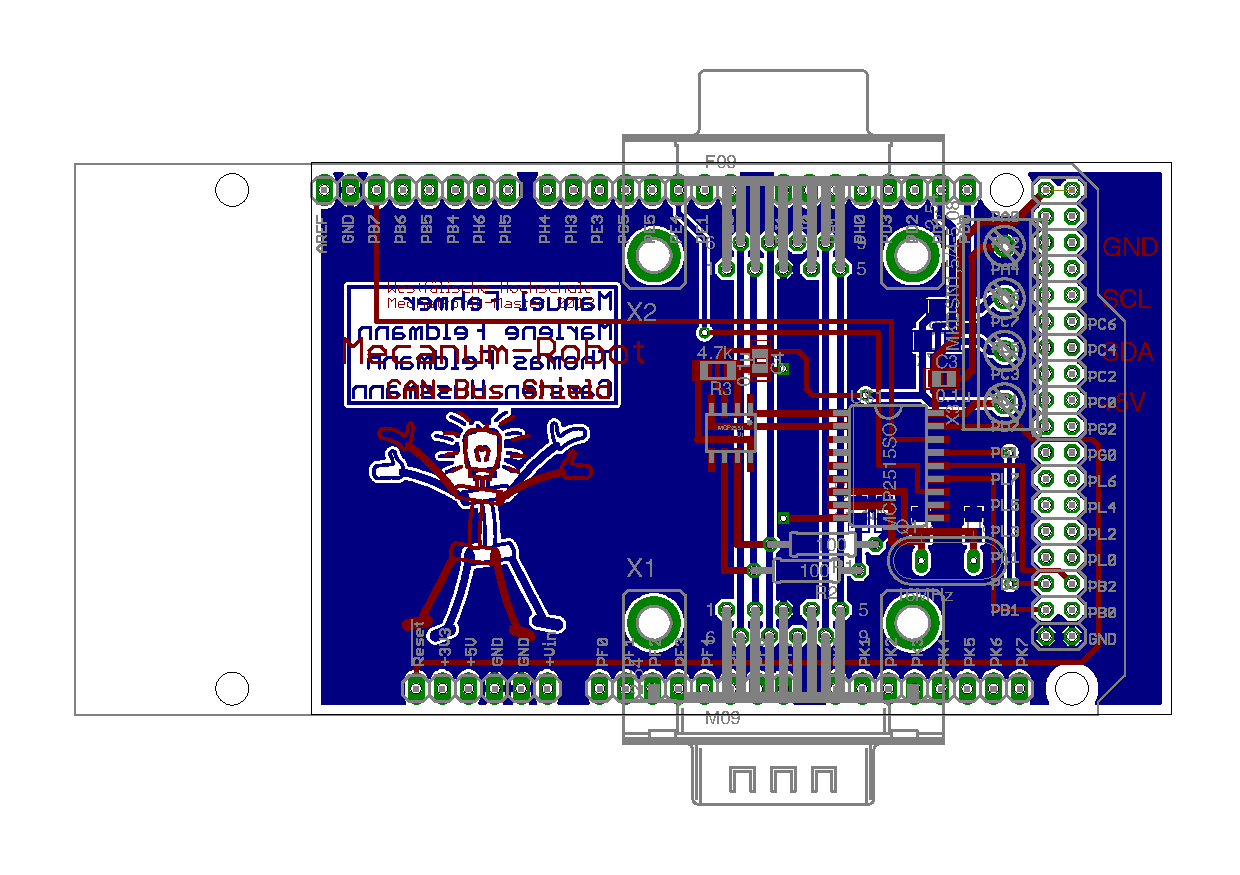
\includegraphics[width=0.8\textwidth]{Abbildungen/CAN-Shield-Layout}
\caption[CAN-Shield-Layout]{CAN-Shield-Layout}
\label{fig:CAN-Shield-Layout}
\end{figure}

\begin{figure}[H]
\centering
 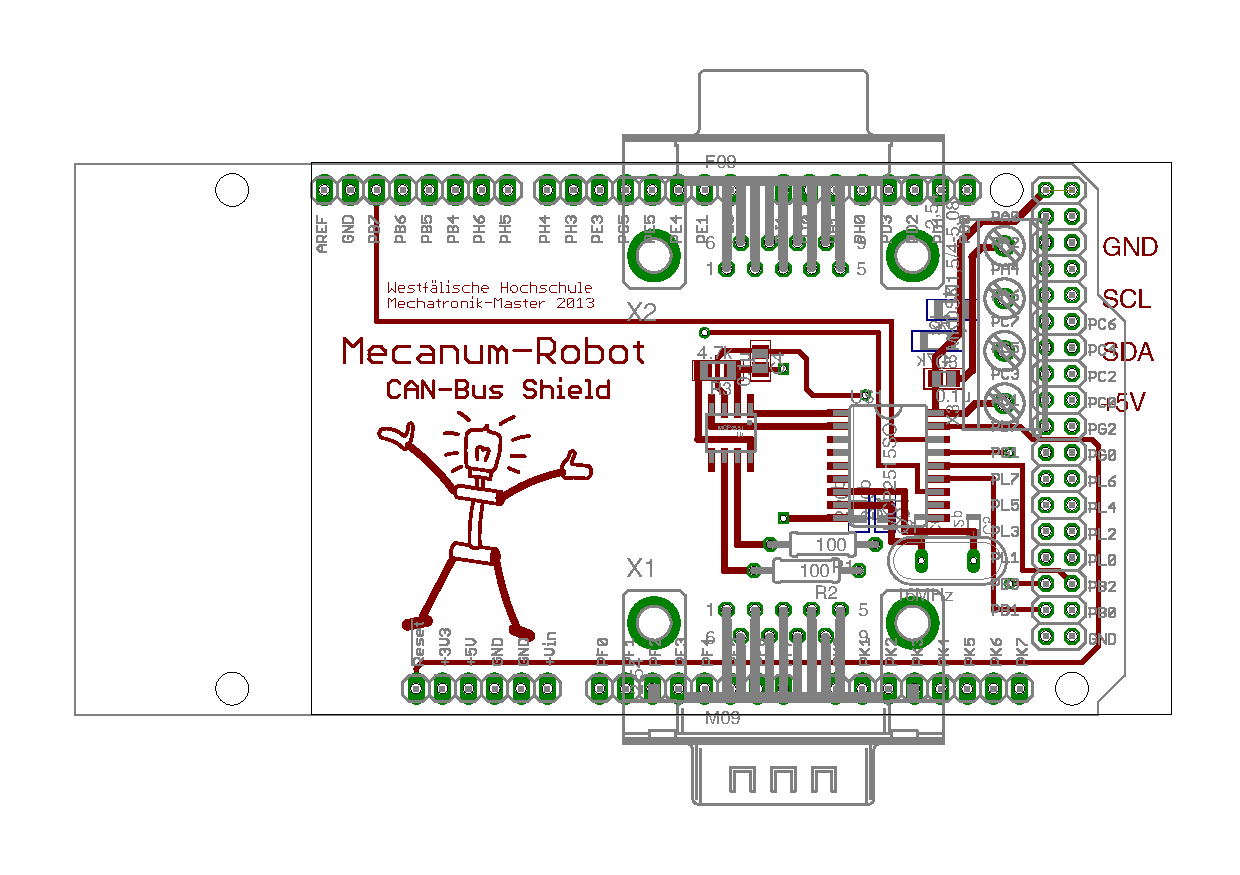
\includegraphics[width=0.8\textwidth]{Abbildungen/CAN-Shield-Layout-Top}
\caption[CAN-Shield-Top-Layer]{CAN-Shield-Top-Layer}
\label{fig:CAN-Shield-Layout-Top}
\end{figure}

\begin{figure}[H]
\centering
 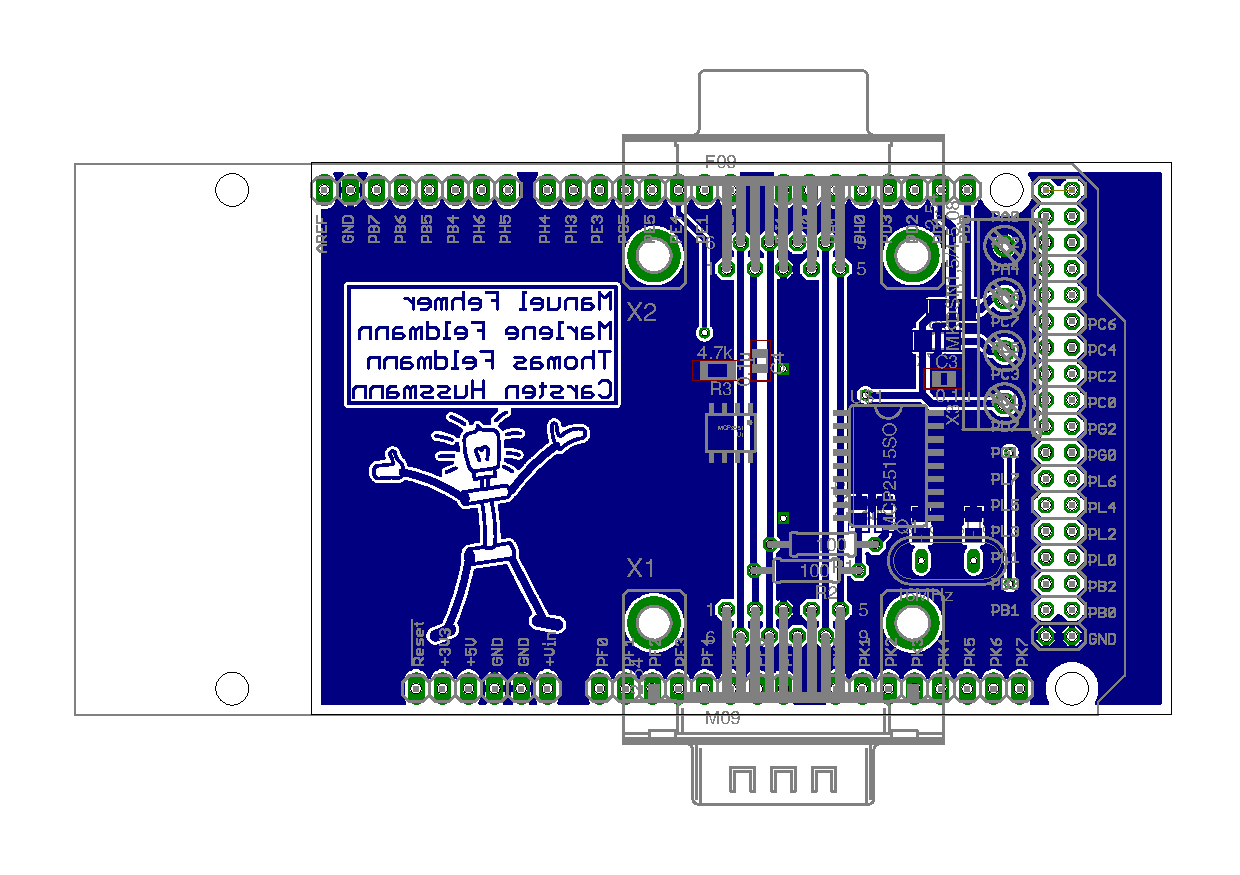
\includegraphics[width=0.8\textwidth]{Abbildungen/CAN-Shield-Layout-Bottom}
\caption[CAN-Shield-Bottom-Layer]{CAN-Shield-Bottom-Layer}
\label{fig:CAN-Shield-Layout-Bottom}
\end{figure}

\subsection{Drahtlose Navigation auf dem Betriebsgelände}
\label{sec:Navigation}
\begin{figure}
\centering
    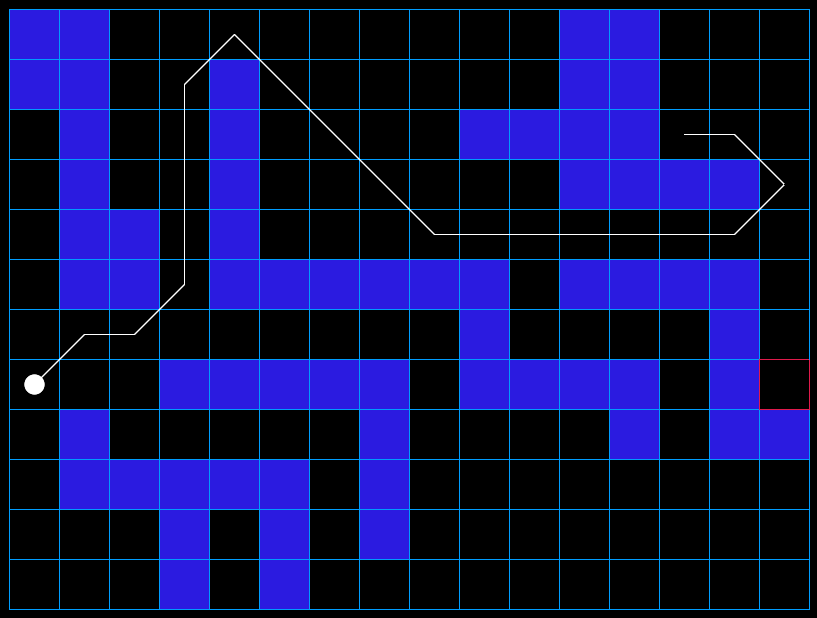
\includegraphics[width=.8\textwidth]{Abbildungen/Dijkstra}
    \caption[Dijkstra]{Pathfinding-Algorithmus nach Dijkstra}
    \label{fig:Dijkstra}
\end{figure}
Um die Navigation auf dem Betriebsgelände zu ermöglichen, muss der Roboter stets seine Position und Ausrichtung im Raum kennen. Dazu kann eine Deckenkamera und eine entsprechende Markierung auf dem Roboter eingesetzt werden.

In Abbildung~\ref{fig:Dijkstra} ist ein Ergebnis des Dijkstra Pathfinding Algorithmus\footnote{http://www.smellycatcards.com/index.php/welcome/pathfinding} dargestellt.
Das Betriebsgelände wird hier in befahrbare (schwarz) und nicht befahrbare Bereiche (blau) eingeteilt. Die resultierende Fahrtvorgabe (weiße Linie) ist die kürzeste Verbindung zwischen Start- und Zielpunkt in der Halle (Ob nur senkrechte oder auch diagonale Fahrten zugelassen werden, kann in der der Implementierung des Algorithmus angepasst werden).

Die nicht befahrbaren Bereiche können auf diese Weise dynamisch angepasst werden. So können auch die Deckenkamera und die auf dem Roboter integrierten Sensoren zur Hindernisserkennung hinzugezogen werden.

Der Roboter soll sich im Akkubetrieb kabellos bewegen können. Für die Kommunikation ist daher die Einrichtung eines Funknetzwerks nötig. Dies kann durch ein auf den Arduino aufgestecktes Ethernet-Shield realisiert werden, wegen der begrenzten Rechenleistung und Speicherkapazität des Arduinos wird diese Möglichkeit aber unnötig kompliziert.
Einfacher wäre die Integration eines Kleinrechners auf Basis von Embedded Linux\footnote{Beispielsweise dem Raspberry Pi: http://www.raspberrypi.org}. Die Server-Framework \emph{Flask\footnote{http://flask.pocoo.org}} auf Basis der Programmiersprache \emph{Python\footnote{http://www.python.org}} stellt eine einfache Möglichkeit dar, den Roboter über ein Webinterface zugänglich zu machen. Über die Library \emph{PySerial\footnote{http://pyserial.sourceforge.net}} kann die in Kapitel~\ref{sec:API} erläuterte API genutzt werden, am Arduino und dem CAN-Bus Shield wären somit keine Änderung notwendig.


